\documentclass[11pt,a4paper]{article}

% ─── Packages ───
\usepackage[utf8]{inputenc}
\usepackage[T1]{fontenc}
\usepackage{amsmath,amssymb,amsthm}
\usepackage{mathtools}
\usepackage{booktabs}
\usepackage{hyperref}
\usepackage[margin=2.5cm]{geometry}
\usepackage{graphicx}
\graphicspath{{figures/}}
\usepackage{caption}
\usepackage{natbib}
% \usepackage{microtype} % enable on local machine for better typography

% ─── Notation shortcuts ───
\newcommand{\RN}{R(N)}
\newcommand{\MN}{M(N)}
\newcommand{\mN}{m(N)}
\newcommand{\wN}{w(N)}
\newcommand{\IN}{I_N(k)}
\newcommand{\Qmax}{Q_{\max}}
\DeclareMathOperator{\atantwo}{atan2}

% ─── Metadata ───
\title{Computational Observations on the Complex-Plane Anatomy\\of Goldbach Major/Minor Arc Decompositions}
\author{Leonardo Germoni}
\date{Draft --- March 2026}

\begin{document}
\maketitle

% ═══════════════════════════════════════
% ABSTRACT
% ═══════════════════════════════════════

\begin{abstract}
The Hardy--Littlewood circle method decomposes a von~Mangoldt weighted binary Goldbach convolution into major and minor arc contributions, which are traditionally analysed separately. As Tao~(2012) observes, in the binary case the minor arc contribution can potentially dominate ``if all one is given about the minor arc sums is magnitude information.'' Motivated by this observation, the present study examines a fixed-$\Qmax$, discrete-grid proxy to this decomposition, retaining phase information and computing the signed contributions from both arc regions empirically, across windows of even integers at scales up to~$10^9$.

After correcting for a major-arc aperture effect identified during the study, the decomposition exhibits a consistent geometric structure in the complex plane across the tested scales, with moderate positive correlation ($r \approx +0.67$ to $+0.73$, converged) and substantial cancellation at large~$N$. The complex diagnostic $\wN = \MN + i \cdot \mN$, where $\MN$ and $\mN$ denote the major and minor arc contributions respectively, reveals tight angular concentration, modular family structure reminiscent of the banding seen in Goldbach's comet, and data consistent with a crossover from a major-dominated to a cancellation-dominated regime.

Simple mechanical models based on the constraint $\MN + \mN = \RN$ predict strong negative correlation ($r \approx -1$); the observed positive correlation differs in sign from all such models. The identification and correction of a measurement artefact, with the observed geometric structure persisting after the correction, constitutes the principal methodological contribution.

These findings are purely empirical and do not constitute a proof of the Goldbach conjecture. They are offered as computational observations on the spectral anatomy of the Goldbach integrand.
\end{abstract}

% ═══════════════════════════════════════
% SECTION 1
% ═══════════════════════════════════════

\section{Introduction}

\subsection{The binary Goldbach problem and the circle method}

The strong Goldbach conjecture asserts that every even integer $N \geq 4$ can be expressed as the sum of two primes. Despite computational verification to approximately $4 \times 10^{18}$ \citep{OliveiraSilva2014} and extensive theoretical progress on related problems, the conjecture remains open.

The Hardy--Littlewood circle method provides the standard analytic framework for studying binary additive problems involving primes. For even~$N$, the von~Mangoldt weighted convolution is expressed as
\begin{equation}\label{eq:RN}
\RN = \int_0^1 S(\alpha)^2\, e(-N\alpha)\, d\alpha
\end{equation}
where $S(\alpha) = \sum_{n \leq N} \Lambda(n)\, e(n\alpha)$ is the prime exponential sum, $\Lambda$ denotes the von~Mangoldt function, and $e(x) = e^{2\pi i x}$. The value $\RN$ equals $\sum_{m+n=N} \Lambda(m)\Lambda(n)$, which is the von~Mangoldt weighted convolution associated with Goldbach-type representations. Positivity of $\RN$ guarantees a representation by integers carrying von~Mangoldt weight, and prime representations contribute positively as a distinguished subset. We work throughout with this weighted object rather than the raw prime-pair count~$g(N)$.

The unit interval $[0,1]$ is partitioned into \emph{major arcs}---neighbourhoods of rationals $a/q$ with small denominator~$q$---and \emph{minor arcs}, the complement. This yields a decomposition
\begin{equation}\label{eq:decomp}
\RN = \MN + \mN
\end{equation}
where $\MN$ and $\mN$ denote the major and minor arc contributions respectively. On the major arcs, $S(\alpha)$ is well approximated by character sums, yielding the Hardy--Littlewood prediction $\MN \approx \mathfrak{S}(N) \cdot N$, where $\mathfrak{S}(N)$ is the singular series. On the minor arcs, one seeks bounds on $|S(\alpha)|$ or averaged estimates.

For the ternary Goldbach problem (sums of three primes), the cubic power in $\int S(\alpha)^3\, e(-N\alpha)\, d\alpha$ ensures the major arc contribution dominates, enabling \citet{Helfgott2013} to give a complete proof. For the binary problem, the situation is fundamentally different. The minor arc $L^2$ mass $\int_{\text{minor}} |S(\alpha)|^2\, d\alpha$ is of order $N \log N$, while the major arc main term is of order~$N$. The minor arcs are larger by a factor of $\log N$ in magnitude, a gap that grows with~$N$ and contributes to the central analytic difficulty.

We emphasise that no claim regarding the Goldbach conjecture is made; the scope of this study is empirical throughout.


\subsection{Motivation: the phase information gap}

The difficulty of the binary Goldbach problem via the circle method is intimately connected to an information loss problem. \citet{Tao2012} identifies three principal obstacles: the magnitude dominance of the minor arcs, the indistinguishability of primes from certain ``redacted'' sets under magnitude-only bounds, and the absence of suitable inverse theorems.

The first of these obstacles carries a crucial qualification. As Tao notes, the minor arc contribution potentially dominates ``if all one is given about the minor arc sums is magnitude information.'' Standard analytic approaches necessarily discard the phase of $S(\alpha)^2 e(-N\alpha)$ on the minor arcs to obtain usable bounds, retaining only magnitude estimates of the form $|S(\alpha)| \leq f(N, \alpha)$. This phase information---the signed, complex-valued structure of the integrand at each frequency---is not directly accessible through magnitude-based bounds.

The standard approach analyses $\MN$ and $\mN$ separately; their joint behaviour across nearby values of~$N$ is not typically studied. The present work asks a different question: when phase information is retained and the signed major and minor arc contributions are computed for a window of even integers around a given~$N$, what empirical relationship do they exhibit?


\subsection{The $w$-plane diagnostic}

To organise the empirical observations, we introduce a complex-valued diagnostic. For each even~$N$ in a scan window, define
\begin{equation}\label{eq:wplane}
\wN = \MN + i \cdot \mN
\end{equation}
where $\MN$ and $\mN$ are the signed (real-valued) major and minor arc contributions satisfying $\MN + \mN = \RN$. In this representation:
\begin{itemize}
\item The real part $\operatorname{Re}(w)$ encodes the major arc contribution.
\item The imaginary part $\operatorname{Im}(w)$ encodes the minor arc contribution.
\item The total weighted count is $\RN = \operatorname{Re}(w) + \operatorname{Im}(w)$.
\item The line $\operatorname{Re} + \operatorname{Im} = 0$ corresponds to $\RN = 0$ for the weighted convolution studied here. This is not identical to the statement of strong Goldbach, but provides a natural geometric reference line for the present computations.
\end{itemize}

The cloud of $\wN$ values across a scan window provides a convenient geometric representation of the decomposition's structure at a given scale. Tight angular clustering suggests a stable geometric relationship between $\MN$ and $\mN$ over the sampled window. The distance from each $\wN$ to the line $\operatorname{Re} + \operatorname{Im} = 0$ provides a per-$N$ measure of how far the weighted convolution sits from zero at each even integer.


\subsection{Summary of findings}

The principal findings of this study, all stated as empirical observations, are as follows.

First, the signed major and minor arc contributions exhibit moderate positive correlation across windows of nearby even integers. At converged arc neighbourhood width (half-width 20 grid points), the Pearson correlation is $r \approx +0.73$ at $N = 10^7$, $r \approx +0.69$ at $N = 10^8$, and $r \approx +0.67$ at $N = 10^9$. This interpretation is based on three scales and should be regarded as suggestive.

Second, simple mechanical models based on the identity $\MN + \mN = \RN$ predict strong negative correlation ($r \approx -1$), whereas the observed correlation is positive. This sign reversal persists across all tested scales in the present computations and is verified by four independent negative controls and one positive control (calibration) experiment.

Third, the $w$-plane diagnostic reveals tight angular concentration that increases with scale in the sampled windows, with the angular standard deviation decreasing from $2.6^\circ$ at $10^7$ to $0.5^\circ$ at $10^9$. The modular families $N \equiv 0 \pmod{6}$ and $N \equiv 2, 4 \pmod{6}$ appear as distinct angular clusters, reproducing the banding seen in Goldbach's comet within the $w$-plane representation.

Fourth, the data are consistent with a crossover from a near-axis, major-dominated regime at $10^7$ (where major/total $\approx 1.0$) to a tightly cancellation-dominated regime at $10^9$ (where major/total $\approx 24.8$, meaning both $|M|$ and $|m|$ are approximately 25 times the total $\RN$). This interpretation is based on three scales and should be regarded as suggestive.

Fifth, an initial measurement artefact was identified during the study: narrow arc neighbourhoods ($\pm 2$ grid points) amplify the measured correlation relative to wider, converged neighbourhoods ($\pm 20$ grid points). The correlation decreased from $r \approx 0.83$ to $r \approx 0.67$ upon correction. The observed geometric structure persisted after this correction. The identification and correction of this aperture effect, with the principal findings persisting in weakened but qualitatively unchanged form, constitutes a methodological contribution applicable to any grid-based arc diagnostic.

Recent explicit work on Goldbach summatory functions emphasises the role of oscillatory zero terms in weighted Goldbach averages \citep{BhowmikHalupczok2018, BhowmikErnvallPalojarvi2025}. The present computations are best viewed as an empirical, phase-retaining probe of related structure at the level of the circle-method decomposition. Whether the observed geometric structure reflects oscillatory zero contributions remains an open question.


% ═══════════════════════════════════════
% SECTION 2
% ═══════════════════════════════════════

\section{Computational Framework}

\subsection{The weighted convolution on a discrete grid}

For a given even integer~$N$, we compute the von~Mangoldt weighted convolution
\begin{equation}
\RN = \sum_{m+n=N} \Lambda(m)\Lambda(n)
\end{equation}
directly, where $\Lambda(n) = \log p$ if $n = p^k$ for some prime~$p$ and integer $k \geq 1$, and $\Lambda(n) = 0$ otherwise. Primes are generated by sieve, and $\Lambda$ is then assigned by marking all prime powers up to the required bound.

To decompose $\RN$ into major and minor arc contributions, we work with the discrete Fourier transform of the $\Lambda$-sequence. Let $N_{\max}$ be the largest integer in the scan window. Define $L = 2N_{\max} + 1$ and consider the $L$-point DFT in the standard (negative-exponent) convention used by \texttt{numpy.fft} and the Goertzel algorithm:
\begin{equation}\label{eq:dft}
F(k) = \sum_{n=0}^{L-1} \Lambda(n)\, e^{-2\pi i n k / L}, \quad k = 0, 1, \ldots, L-1.
\end{equation}

Since the $\Lambda$-sequence has support in $[0, N_{\max}]$ and $L > 2N_{\max}$, the circular convolution computed by the DFT agrees with the linear convolution for all~$N$ in the scan window, avoiding wrap-around artefacts.

The weighted convolution $\RN$ can be recovered from these DFT coefficients:
\begin{equation}\label{eq:recovery}
\RN = \frac{1}{L} \sum_{k=0}^{L-1} F(k)^2\, e^{2\pi i N k / L}.
\end{equation}

The phase-retaining integrand at each grid frequency is therefore
\begin{equation}\label{eq:integrand}
\IN = \frac{1}{L}\, F(k)^2\, e^{2\pi i N k / L}
\end{equation}
so that $\RN = \sum_k \IN$. Once the discrete grid and major index set are fixed, the decomposition is exact on that grid at the algebraic level, up to floating-point rounding in implementation. The grid decomposition is not identical to the continuous arc decomposition of the Hardy--Littlewood method; it is a finite computational proxy designed to retain phase information on a discrete frequency set.

In the classical Hardy--Littlewood formulation, major arcs are neighbourhoods of width approximately $Q/N$ around rationals $a/q$ with $q \leq Q$, where $Q$ grows with~$N$ (typically $Q = N^\delta$ for some $\delta > 0$). In the present discrete setting, $\Qmax = 20$ is held fixed across all scales, and the neighbourhood width is controlled by the half-width parameter $\mathrm{hw}$ in grid points. At $N = 10^9$, the classical choice $Q = N^{1/6} \approx 31$ is comparable to the fixed $\Qmax = 20$ used here; the $\Qmax$ sensitivity analysis (\S5.1) confirms stability of the measured correlation across $\Qmax$ values from 10 to 50. The convergence analysis in~\S\ref{sec:convergence} demonstrates internal stability: the measured quantities are insensitive to $\mathrm{hw}$ once it is large enough to capture the full peak around each rational centre. This is a statement about the discrete grid decomposition, not a proof of convergence to the classical continuous arc decomposition. The extent to which the discrete proxy at fixed $\Qmax$ approximates the continuous theory---particularly for contributions from rationals with $q > \Qmax$---is a limitation of the present approach.


\subsection{Major and minor arc classification}

The unit circle $[0,1)$ is discretised into $L$ equally spaced frequencies $\alpha_k = k/L$. We classify each frequency as belonging to a major or minor arc based on its proximity to rationals with small denominator. Throughout this paper, the terms ``major arc'' and ``minor arc'' refer exclusively to this discrete-grid classification with fixed~$\Qmax$, not to the classical continuous decomposition of the Hardy--Littlewood circle method, in which the arc parameters typically grow with~$N$.

Define the circular distance on $\{0, 1, \ldots, L-1\}$ as
\begin{equation}
d_L(k, \ell) = \min(|k - \ell|,\; L - |k - \ell|).
\end{equation}

For parameters $\Qmax$ (the maximum denominator) and $\mathrm{hw}$ (the half-width in grid points), a frequency index~$k$ is classified as major if there exist integers $a, q$ with $1 \leq q \leq \Qmax$, $0 \leq a < q$, $\gcd(a,q) = 1$, such that
\begin{equation}
d_L\!\bigl(k,\; \operatorname{round}(aL/q)\bigr) \leq \mathrm{hw}.
\end{equation}

The major index set $I_{\mathrm{maj}}$ is formed as the union of all such neighbourhoods, with overlaps removed. All other indices are classified as minor.

The major and minor arc contributions for a given~$N$ are
\begin{align}
\MN &= \sum_{k \in I_{\mathrm{maj}}} \IN, \\
\mN &= \RN - \MN.
\end{align}

Because the major index set is symmetric under $k \to L - k$, the summed contributions are real up to floating-point error; in implementation, residual imaginary parts were numerically negligible.

The minor arc contribution is defined as the exact residual, ensuring $\MN + \mN = \RN$ by construction. This avoids accumulation of rounding errors in the minor arc sum.

Throughout this study, $\Qmax = 20$ is used. The half-width parameter $\mathrm{hw}$ is varied from 2 to 20 grid points as part of the convergence analysis described in~\S\ref{sec:convergence}. At $\mathrm{hw} = 20$, the number of distinct major-arc grid points (after deduplication) is approximately 5{,}248 out of $L \approx 2 \times 10^9$ at $N = 10^9$.


\subsection{Computational methods}

Two methods are employed to evaluate the DFT coefficients at the major-arc frequencies, depending on the scale~$N$.

\paragraph{FFT method ($N \leq 10^8$).}
The full $L$-point DFT is computed using \texttt{numpy.fft}, which implements the negative-exponent convention matching~\eqref{eq:dft}. The total $\RN$ is obtained via the inverse FFT, and the major-arc contribution $\MN$ is computed by summing $\IN$ over the major indices $I_{\mathrm{maj}}$. Memory requirements are feasible on the available hardware for $L$ up to approximately $2 \times 10^8$, but not for $L \approx 2 \times 10^9$.

\paragraph{Goertzel method ($N = 10^9$).}
At $N = 10^9$, the DFT length $L \approx 2 \times 10^9$ exceeds available memory for a full FFT. Instead, individual DFT bins $F(k)$ are computed using the standard Goertzel recurrence, which evaluates a single bin in $O(L)$ time and $O(1)$ space. The recurrence is implemented with \texttt{numba} just-in-time compilation for performance. Parallelism across major-arc frequencies is achieved using Python's \texttt{multiprocessing} module with 12 worker processes.

The total $\RN$ at each scan point is computed independently via the inner product
\begin{equation}
\RN = \sum_{j=1}^{N-1} \Lambda(j)\,\Lambda(N-j)
\end{equation}
implemented as a \texttt{numpy} dot product of array views.

\paragraph{Cross-validation.}
At $N = 10^7$ and $N = 10^8$, where both FFT and Goertzel are feasible, the two methods agree within relative error $< 10^{-7}$ in the major-arc contribution and $< 10^{-10}$ in the total. This provides confidence that the Goertzel implementation at $N = 10^9$ is correct.


\subsection{Scan windows and sampling}

For each target scale $N_{\mathrm{center}}$, a scan window of 201 evenly spaced even integers is evaluated:
\begin{equation}
N \in \{N_{\mathrm{center}} - 2000,\; N_{\mathrm{center}} - 1980,\; \ldots,\; N_{\mathrm{center}} + 2000\}
\end{equation}
with step size~20. The window width ($\pm 2000$) is small relative to $N_{\mathrm{center}}$ (less than $0.0004\%$ at $10^9$), so the DFT length~$L$ and the major-arc index set $I_{\mathrm{maj}}$ are effectively constant across the window. Variation in $\MN$ and $\mN$ across the window arises from the $N$-dependent twist factor $e^{2\pi i N k / L}$ in the integrand $\IN$, not from changes in the grid geometry.

Three target scales are examined: $N_{\mathrm{center}} = 10^7$, $10^8$, and $10^9$. The upper limit is set by hardware: at $N = 10^9$ each scan window requires approximately 80 minutes of Goertzel computation on a 12-core workstation with 48\,GB RAM, and memory constraints preclude a full FFT at this scale.


\subsection{Convergence in half-width}\label{sec:convergence}

The half-width parameter $\mathrm{hw}$ controls the number of grid points assigned to each major-arc neighbourhood. In the present discretisation, the operational neighbourhood width chosen to capture a full peak around each selected rational centre is approximately 40 grid points. The half-width $\mathrm{hw}$ determines what fraction of this operational width is captured:
\begin{itemize}
\item At $\mathrm{hw} = 2$ (5 grid points per centre, 640 major indices total), each neighbourhood is narrow relative to the peak structure, constituting substantial undersampling.
\item At $\mathrm{hw} = 5$ (11 grid points, 1{,}408 indices), coverage is partial.
\item At $\mathrm{hw} = 10$ (21 grid points, 2{,}688 indices), coverage is approximately half.
\item At $\mathrm{hw} = 20$ (41 grid points, 5{,}248 indices), the neighbourhood slightly exceeds the nominal width, ensuring full coverage of the selected neighbourhood around each rational centre.
\end{itemize}

The major/total fraction $\MN/\RN$ converges as $\mathrm{hw}$ increases. At $N = 10^7$, it evolves from $+0.92$ ($\mathrm{hw} = 2$) to $+1.00$ ($\mathrm{hw} = 20$); at $N = 10^8$, from $+0.78$ to $+0.86$; at $N = 10^9$, from $-13.9$ to $+24.8$. The sign reversal at $N = 10^9$ with $\mathrm{hw} = 2$ is a subsampling artefact: the narrow neighbourhood captures an oscillatory slice of the peak structure whose sign depends on the local phase. Wider neighbourhoods integrate over the full peak and recover the expected positive major-arc contribution.

The Pearson correlation $r(M, m)$ decreases monotonically with $\mathrm{hw}$ at all three scales:

\begin{table}[h]
\centering
\begin{tabular}{l rrrr}
\toprule
$N$ & $\mathrm{hw}=2$ & $\mathrm{hw}=5$ & $\mathrm{hw}=10$ & $\mathrm{hw}=20$ \\
\midrule
$10^7$ & $+0.87$ & $+0.78$ & $+0.75$ & $+0.73$ \\
$10^8$ & $+0.84$ & $+0.75$ & $+0.71$ & $+0.69$ \\
$10^9$ & $+0.83$ & $+0.74$ & $+0.70$ & $+0.67$ \\
\bottomrule
\end{tabular}
\caption{Pearson correlation $r(M,m)$ as a function of half-width $\mathrm{hw}$.}
\label{tab:convergence}
\end{table}

The correlation remains positive at all tested half-widths and scales. The decrease from $\mathrm{hw} = 2$ to $\mathrm{hw} = 20$ reflects the removal of an amplification effect: narrower neighbourhoods preferentially sample the coherent peak centres of the major arcs, inflating the measured correlation. The converged values at $\mathrm{hw} = 20$ are reported as the primary results throughout this paper.

The convergence of the major/total fraction by $\mathrm{hw} = 10$ (with $|\Delta| < 0.01$ between $\mathrm{hw} = 10$ and $\mathrm{hw} = 20$) provides an internal consistency check on the grid resolution. The convergence of the correlation, while not as sharp, shows a clear plateau forming between $\mathrm{hw} = 10$ and $\mathrm{hw} = 20$, supporting the choice of $\mathrm{hw} = 20$ as a stable operating point.

\begin{figure}[ht]
\centering
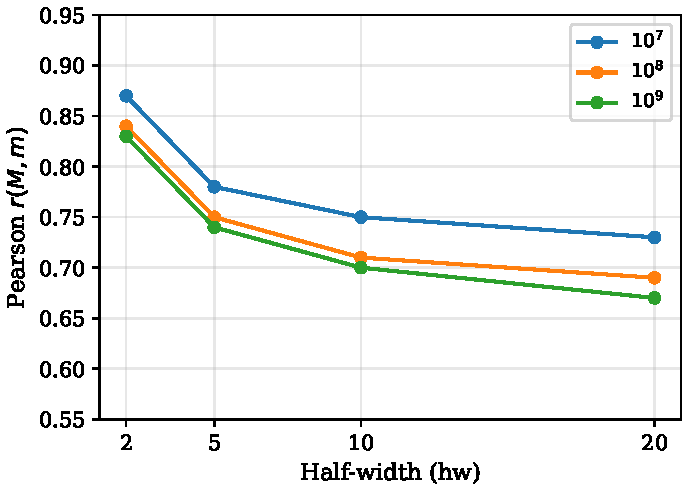
\includegraphics[width=0.55\textwidth]{fig1_convergence.pdf}
\caption{Pearson correlation $r(M,m)$ as a function of half-width $\mathrm{hw}$ at three scales. The correlation decreases monotonically as the arc neighbourhood widens, reflecting the removal of an aperture amplification effect. All values remain positive.}
\label{fig:convergence}
\end{figure}


% ═══════════════════════════════════════
% SECTION 3
% ═══════════════════════════════════════

\section{The $w$-Plane Framework}

\subsection{Definition and basic properties}

For each even integer~$N$ in a scan window, define the complex-valued diagnostic
\begin{equation}
\wN = \MN + i \cdot \mN
\end{equation}
where $\MN$ and $\mN$ are the real-valued major and minor arc contributions defined in~\S2.2. Since $\MN + \mN = \RN$, the weighted convolution is recovered as $\RN = \operatorname{Re}(\wN) + \operatorname{Im}(\wN)$.

The modulus and argument of $\wN$ are
\begin{align}
|\wN| &= \sqrt{\MN^2 + \mN^2}, \\
\arg(\wN) &= \atantwo(\mN, \MN)
\end{align}
where $\atantwo$ denotes the two-argument arctangent, which preserves quadrant information. The modulus $|\wN|$ measures the overall scale of the two-component decomposition, while $\arg(\wN)$ measures the angular balance between major and minor arc contributions.


\subsection{The counterexample reference line}

A hypothetical even integer~$Z$ with $R(Z) = 0$ for the weighted convolution would satisfy $\operatorname{Re}(w(Z)) + \operatorname{Im}(w(Z)) = 0$, corresponding to the line $m = -M$ in the $w$-plane, or equivalently the line through the origin at angle $3\pi/4$ (in the second quadrant) and $-\pi/4$ (in the fourth quadrant). We refer to this as the \emph{reference line}. We emphasise that $R(Z) = 0$ for the weighted convolution is not identical to the statement that $Z$ is a Goldbach counterexample, since $\RN$ includes prime-power contributions (see~\S1.1). The reference line is used here as a geometric landmark, not as a direct proxy for the Goldbach conjecture.

The signed perpendicular distance from $\wN$ to this reference line is
\begin{equation}
\delta(N) = \frac{\MN + \mN}{\sqrt{2}} = \frac{\RN}{\sqrt{2}}
\end{equation}
which is positive whenever $\RN > 0$.


\subsection{Angular concentration and regime classification}

In a \emph{major-dominated regime}, $\MN$ is positive and much larger than $|\mN|$. The $\wN$ cloud lies near the positive real axis with moderate angular spread.

In a \emph{cancellation-dominated regime}, both $|\MN|$ and $|\mN|$ are much larger than $\RN$, and $\RN$ is a small residual of two large, nearly opposing terms. In this regime, the angular spread may be very tight because the ratio $\MN/\mN$ is approximately constant across the window, suggesting that both components are responding to a common large-scale pattern in the decomposition.

Whether such a transition is a continuous crossover or a sharper change cannot be determined from the present data alone.


\subsection{Modular family structure}

The Hardy--Littlewood singular series $\mathfrak{S}(N)$ depends on the prime factorisation of~$N$, creating systematic variation in $\RN$ across arithmetic families. The most prominent effect is the mod~6 classification: $\mathfrak{S}(N)$ is larger for $N \equiv 0 \pmod{6}$ than for $N \equiv 2$ or $4 \pmod{6}$. This is the origin of the two-band structure visible in Goldbach's comet.

In the $w$-plane, this modular structure manifests as distinct clusters within the cloud. Points with $N \equiv 0 \pmod{6}$ are observed to have larger $|\wN|$ and occupy a slightly different angular position than points with $N \equiv 2$ or $4 \pmod{6}$ in the present data.


\subsection{Connection to existing theory}

The $w$-plane diagnostic is an empirical construction; it does not arise from a theorem or a standard decomposition in the analytic number theory literature.

The Goldbach summatory function $S(x) = \sum_{n \leq x} G(n)$, where $G(n)$ denotes the von~Mangoldt weighted Goldbach convolution, satisfies, under the Riemann Hypothesis,
\begin{equation}
S(x) = \frac{x^2}{2} - H(x) + \text{error terms}
\end{equation}
where $H(x) = -2\sum_\rho x^{\rho+1}/(\rho(\rho+1))$ is an oscillatory term summed over the non-trivial zeros~$\rho$ of the Riemann zeta function \citep{Fujii1991, Granville2007, BhowmikHalupczok2018}. Recent explicit work has obtained unconditional numerical estimates for these summatory functions \citep{BhowmikErnvallPalojarvi2025}.

The individual-$N$ behaviour of $\MN$ and $\mN$ may plausibly reflect some of the same oscillatory phenomena that contribute to $H(x)$, though at a much finer and unsmoothed level. Whether the observed geometric structure in the $w$-plane reflects oscillatory zero structure is a natural question, but one the present study does not resolve.


% ═══════════════════════════════════════
% SECTION 4
% ═══════════════════════════════════════

\section{Empirical Results}

All results in this section are reported at the converged half-width $\mathrm{hw} = 20$ unless otherwise stated. The reported values summarise each 201-point window.

\subsection{Signed correlation across scales}

\begin{table}[h]
\centering
\begin{tabular}{l cc c}
\toprule
$N_{\mathrm{center}}$ & $r$ ($\mathrm{hw}=20$) & Spearman $\rho$ & $n$ \\
\midrule
$10^7$ & $+0.73$ & $+0.69$ & 201 \\
$10^8$ & $+0.69$ & $+0.64$ & 201 \\
$10^9$ & $+0.67$ & $+0.62$ & 201 \\
\bottomrule
\end{tabular}
\caption{Pearson and Spearman correlations between $\MN$ and $\mN$.}
\label{tab:correlation}
\end{table}

The sampled values within a narrow window are not independent draws from a stationary distribution, so standard parametric $p$-values are not valid under this sampling design. Evidence for the robustness of the correlation is instead provided by permutation tests, bootstrap confidence intervals, and block bootstrap, reported in~\S5.

The correlation is positive at all three scales. The values decrease gently from $+0.73$ to $+0.67$ across two orders of magnitude in~$N$, but with only three scales this should be viewed as a descriptive observation rather than evidence of asymptotic behaviour.


\subsection{$w$-plane geometry}

The $\wN$ cloud at each scale is concentrated in a distinct region of the complex plane. Since the angle clusters are narrow and remain far from the branch cut, ordinary and circular summaries are numerically indistinguishable in the sampled windows.

\begin{table}[h]
\centering
\begin{tabular}{l ccc}
\toprule
Quantity & $N = 10^7$ & $N = 10^8$ & $N = 10^9$ \\
\midrule
Mean $\operatorname{Re}(w)$ & $2.47 \times 10^7$ & $2.15 \times 10^8$ & $5.58 \times 10^{10}$ \\
Mean $\operatorname{Im}(w)$ & $2.54 \times 10^5$ & $3.55 \times 10^7$ & $-5.33 \times 10^{10}$ \\
Mean angle & $-0.0^\circ$ & $+9.7^\circ$ & $-43.7^\circ$ \\
Angular std & $2.6^\circ$ & $2.3^\circ$ & $0.5^\circ$ \\
Quadrant dist. & Q1:44\%, Q4:56\% & Q1:100\% & Q4:100\% \\
Min $\delta(N)$ & $1.24 \times 10^7$ & $1.24 \times 10^8$ & $1.24 \times 10^9$ \\
All $\RN > 0$? & Yes & Yes & Yes \\
\bottomrule
\end{tabular}
\caption{Summary of $w$-plane geometry at three scales.}
\label{tab:wplane}
\end{table}

The shift in quadrant distribution follows from the evolution of the mean angle: at $N = 10^7$ the mean angle is near zero and points straddle the real axis; at $10^8$ the mean angle is positive and all points lie in~Q1; at $10^9$ the mean angle is negative and all points lie in~Q4.

\begin{figure}[ht]
\centering
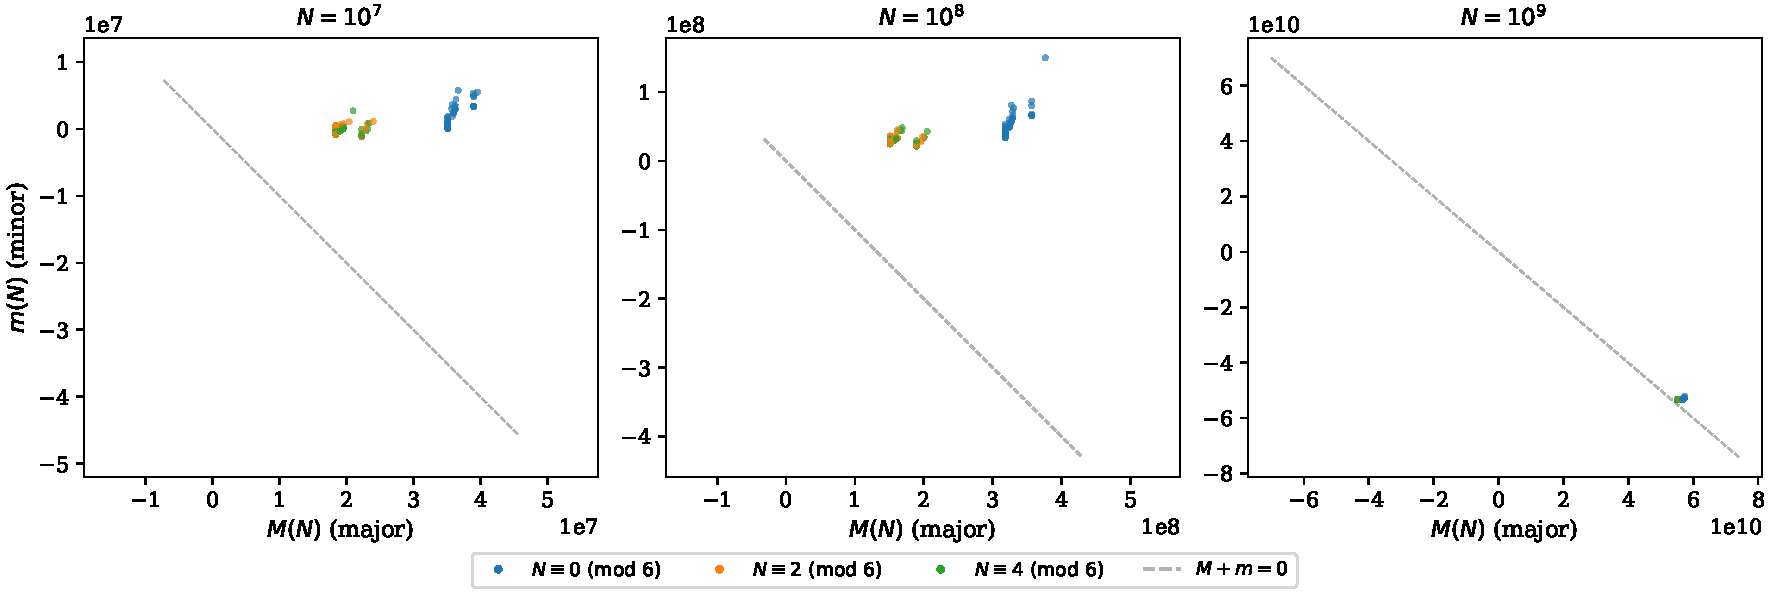
\includegraphics[width=\textwidth]{fig2_wplane.pdf}
\caption{The $w(N)$ cloud at three scales ($\mathrm{hw}=20$). Each point represents one even integer $N$ in the scan window, plotted at $(\MN, \mN)$. Points are coloured by $N \bmod 6$. The dashed line is the reference line $M + m = 0$. Note the change in scale and the rotation of the cloud from near the real axis ($10^7$) to $-43.7^\circ$ ($10^9$).}
\label{fig:wplane}
\end{figure}


\subsection{Major/total fraction and angular concentration}

\begin{table}[h]
\centering
\begin{tabular}{l ccc}
\toprule
$N_{\mathrm{center}}$ & Mean $M/R$ & Std$(M/R)$ & Angular std \\
\midrule
$10^7$ & $+1.003$ & $0.044$ & $2.63^\circ$ \\
$10^8$ & $+0.855$ & $0.030$ & $2.33^\circ$ \\
$10^9$ & $+24.82$ & $6.99$ & $0.47^\circ$ \\
\bottomrule
\end{tabular}
\caption{Major/total fraction and angular concentration.}
\label{tab:fraction}
\end{table}

At $N = 10^7$, the mean major arc contribution is approximately equal to the total. At $N = 10^9$, the major arc contribution is approximately 25 times the total, indicating that both $|\MN|$ and $|\mN|$ are much larger than $\RN$. A ratio $M/R$ substantially greater than~1 does not indicate an inconsistency in the decomposition; it reflects a cancellation regime in which $\MN$ and $\mN$ are large quantities of opposite sign whose sum $\RN$ is a small positive residual.

\begin{figure}[ht]
\centering
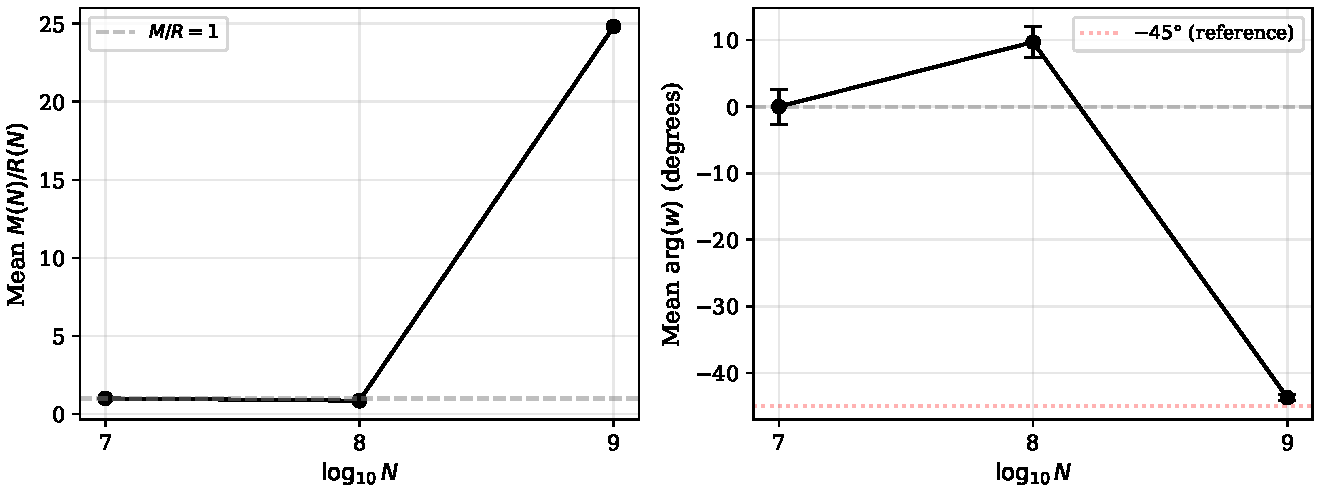
\includegraphics[width=0.85\textwidth]{fig3_regime.pdf}
\caption{Regime indicators at three scales. Left: mean $M(N)/R(N)$ ratio, showing the transition from $\approx 1$ (major-dominated) to $\approx 25$ (cancellation-dominated). Right: mean $\arg(w)$ with angular standard deviation as error bars, showing the rotation of the $w(N)$ cloud away from the real axis.}
\label{fig:regime}
\end{figure}


\subsection{Modular family structure in the $w$-plane}

\begin{table}[h]
\centering
\begin{tabular}{l l cccc}
\toprule
Scale & $N \bmod 6$ & $n$ & Mean angle & Angular std & Mean $|w|$ \\
\midrule
$10^7$ & 0 & 67 & $+2.5^\circ$ & $2.5^\circ$ & $3.60 \times 10^7$ \\
       & 2 & 67 & $-1.3^\circ$ & $1.6^\circ$ & $1.92 \times 10^7$ \\
       & 4 & 67 & $-1.3^\circ$ & $1.6^\circ$ & $1.92 \times 10^7$ \\
\midrule
$10^8$ & 0 & 67 & $+8.5^\circ$ & $2.8^\circ$ & $3.30 \times 10^8$ \\
       & 2 & 67 & $+10.3^\circ$ & $1.7^\circ$ & $1.61 \times 10^8$ \\
       & 4 & 67 & $+10.3^\circ$ & $1.9^\circ$ & $1.62 \times 10^8$ \\
\midrule
$10^9$ & 0 & 67 & $-43.0^\circ$ & $0.2^\circ$ & $7.78 \times 10^{10}$ \\
       & 2 & 67 & $-44.0^\circ$ & $0.1^\circ$ & $7.68 \times 10^{10}$ \\
       & 4 & 67 & $-44.0^\circ$ & $0.1^\circ$ & $7.68 \times 10^{10}$ \\
\bottomrule
\end{tabular}
\caption{Modular family structure in the $w$-plane.}
\label{tab:modular}
\end{table}

At all three scales, the $N \equiv 0 \pmod{6}$ class has larger mean $|w|$ than the other two classes, which are consistent with each other. The angular separation is small but consistent ($1$--$2^\circ$). These separations are reported as descriptive features; no formal significance test on the angular differences has been performed.

\begin{figure}[ht]
\centering
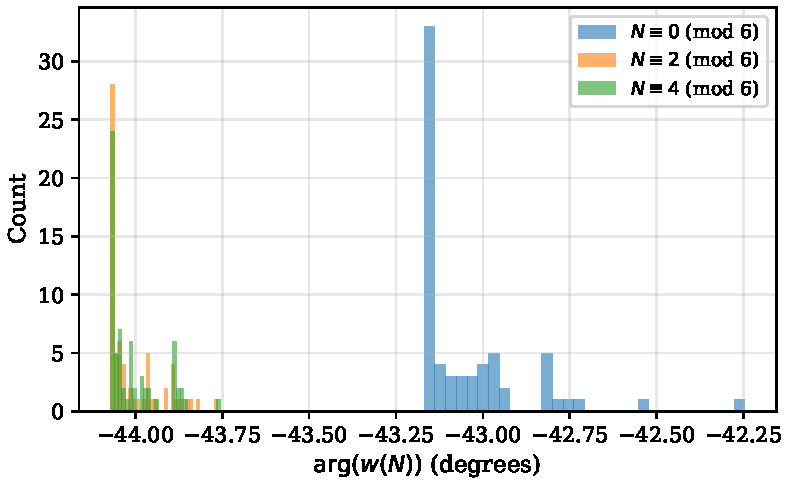
\includegraphics[width=0.65\textwidth]{fig4_modular.pdf}
\caption{Distribution of $\arg(w(N))$ at $N = 10^9$, split by $N \bmod 6$. The three modular families occupy distinct but overlapping angular ranges, with $N \equiv 0 \pmod{6}$ slightly separated from the other two classes.}
\label{fig:modular}
\end{figure}


\subsection{Distance to the reference line}

At all three scales and for all 201 sampled even integers, $\RN > 0$, so $\delta(N) > 0$ and no sampled point lies on or beyond the reference line.

\begin{table}[h]
\centering
\begin{tabular}{l ccc}
\toprule
$N_{\mathrm{center}}$ & Min $\RN$ & Mean $\RN$ & Min $\delta(N)$ \\
\midrule
$10^7$ & $1.75 \times 10^7$ & $2.50 \times 10^7$ & $1.24 \times 10^7$ \\
$10^8$ & $1.75 \times 10^8$ & $2.50 \times 10^8$ & $1.24 \times 10^8$ \\
$10^9$ & $1.75 \times 10^9$ & $2.50 \times 10^9$ & $1.24 \times 10^9$ \\
\bottomrule
\end{tabular}
\caption{Distance to the reference line $\operatorname{Re}+\operatorname{Im}=0$.}
\label{tab:distance}
\end{table}

In the sampled windows, the minimum distance scales approximately proportionally with $N_{\mathrm{center}}$, consistent with the growth of $\RN$ over the tested range.


% ═══════════════════════════════════════
% SECTION 5
% ═══════════════════════════════════════

\section{Validation and Controls}

This section summarises the tests used to assess the robustness of the empirical findings in~\S4. The validation analysis has two purposes: first, to show that the observed positive correlation is not a trivial statistical or algebraic artefact; second, to show that the principal qualitative features persist after convergence correction.


\subsection{Statistical validation of the correlation}

The following tests were applied to the signed correlation $r(M,m)$ at $N = 10^9$ at $\mathrm{hw} = 20$, where the observed Pearson correlation is $r = +0.67$.

\paragraph{Permutation test.} The $\MN$ values were randomly shuffled 10{,}000 times. None of the shuffled replicates equalled or exceeded the observed value. The maximum shuffled correlation was $r = +0.27$.

\paragraph{Bootstrap confidence interval.} 10{,}000 bootstrap resamples yielded a 95\% confidence interval of $[+0.61, +0.76]$ for $r$, with bootstrap mean $+0.68$.

\paragraph{Block bootstrap.} A block bootstrap with block size 20 yielded a 95\% confidence interval of $[+0.62, +0.74]$, consistent with the standard bootstrap.

\paragraph{Split-half reliability.} All four partitions (first/second half, even/odd indices) produced positive correlations in the range $[+0.62, +0.77]$.

\paragraph{Detrending.} Linear detrending produced negligible change ($\Delta r = +0.0001$).

\paragraph{Robust correlation measures.}

\begin{table}[h]
\centering
\begin{tabular}{l c}
\toprule
Measure & Value \\
\midrule
Pearson & $+0.67$ \\
Spearman & $+0.68$ \\
Kendall & $+0.51$ \\
\bottomrule
\end{tabular}
\caption{Robust correlation measures at $\mathrm{hw}=20$, $N=10^9$.}
\label{tab:robust}
\end{table}

All are positive. The Spearman rank correlation slightly exceeds the Pearson value, indicating that the association is not driven by outliers. Nominal parametric $p$-values are not reported because the sampled values are not independent draws from a stationary distribution; the permutation test and bootstrap intervals above provide the appropriate robustness evidence.


\subsection{Mechanical coupling controls}

The identity $\MN + \mN = \RN$ creates an algebraic coupling. To determine whether the observed positive correlation could arise from this constraint alone, five models were tested at $\mathrm{hw} = 2$ and $N = 10^9$. Since the analysis concerns the sign of the correlation, the qualitative conclusions apply regardless of half-width.

Four negative controls (Models A, B, D, E) predict $r \approx -1.0$. At the initial narrow width ($\mathrm{hw} = 2$), all four baselines yield $r \approx -1.0$ against the observed $r = +0.83$, an excess of $+1.83$. At the converged half-width ($\mathrm{hw} = 20$), the sign reversal persists: the observed $r = +0.67$ against the same mechanical prediction of $r \approx -1.0$, giving an excess of approximately $+1.67$. In none of the 40{,}000 total synthetic realisations did the synthetic correlation equal or exceed the observed value at either half-width.

A positive control (Model~C) reproduces the observed correlation to within 0.0003, confirming internal consistency.

\begin{figure}[ht]
\centering
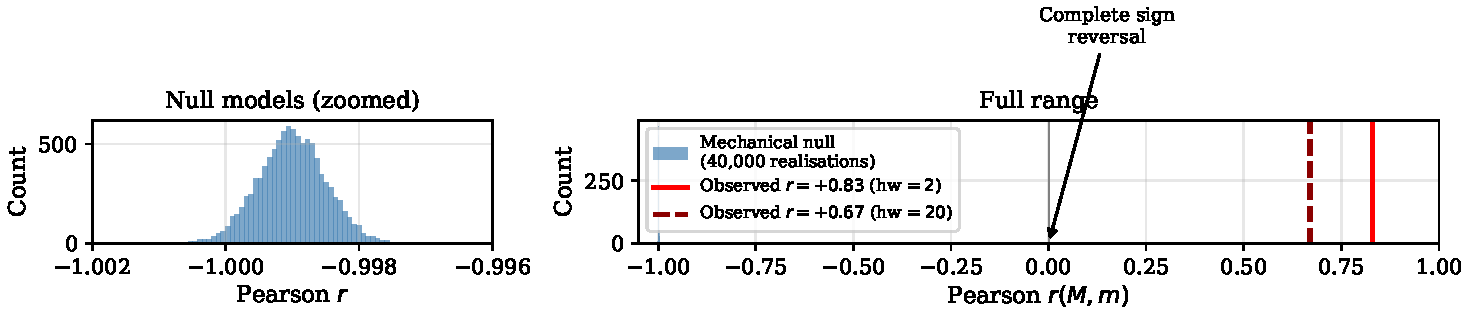
\includegraphics[width=0.65\textwidth]{fig5_mechanical.pdf}
\caption{Distribution of Pearson correlations from 40{,}000 mechanical null-model realisations (Models A, B, E combined), compared with the observed values at $\mathrm{hw} = 2$ (solid red) and $\mathrm{hw} = 20$ (dashed red). The sign reversal is complete: all null realisations cluster near $r \approx -1$, while the observed values are positive.}
\label{fig:mechanical}
\end{figure}


\subsection{Convergence as internal validation}

The initial results at $\mathrm{hw} = 2$ reported $r \approx 0.83$. The convergence analysis revealed this was amplified by the narrow arc neighbourhood; the converged value at $\mathrm{hw} = 20$ is $r \approx 0.67$. The correction weakened the headline number but did not change its sign or qualitative character.

The identification of this aperture amplification effect is itself a methodological contribution. Any future study using grid-based arc diagnostics on additive problems should be aware that narrow neighbourhoods can amplify measured correlations relative to converged values.


\subsection{Cross-method validation}

The computational framework employs two independent methods (\S2.3). At $N = 10^4$ and $10^5$, individual DFT bins computed by FFT and Goertzel agreed to relative error below $10^{-7}$. At $N = 10^7$ and $10^8$, the major/total fraction agrees to better than $10^{-7}$ between methods. The wide-arc computation at $N = 10^9$ was executed twice independently, producing identical reported values and matching output checksums.


\subsection{Falsified hypotheses}

Several hypotheses were tested and rejected:
\begin{itemize}
\item \textbf{Mod~5 bimodal effect.} Apodisation reduced the apparent effect by 99\%; identified as an aperture artefact.
\item \textbf{Mod~6 family differences in correlation.} ANOVA $p = 0.96$; a sampling artefact.
\item \textbf{Universal minor-arc positivity.} At $\mathrm{hw} = 20$, the fraction of positive $\mN$ drops to 44\% at $10^7$ and 0\% at $10^9$.
\item \textbf{$r \approx 0.83$ as the converged correlation.} Amplified by approximately 0.16 relative to the converged value $r \approx 0.67$.
\end{itemize}

Additional falsified hypotheses, including a non-commutative quaternion sieve experiment, are documented in Appendix~D.


\subsection{Code provenance and reproducibility}

Final reported results in this paper are generated from the converged wide-arc pipeline (\texttt{goldbach\_wide\_arc.py}) and its corresponding $\mathrm{hw} = 20$ validation script (\texttt{goldbach\_stats\_hw20.py}). Earlier scripts in the repository reflect development stages associated with narrower arc neighbourhoods and are retained for reproducibility of intermediate analyses documented in~\S5.3 and Appendix~C. All code, cached output data, and checksums are available in the accompanying repository.


% ═══════════════════════════════════════
% SECTION 6
% ═══════════════════════════════════════

\section{Interpretation and Discussion}

\subsection{The observed co-movement}

The most basic empirical observation is that $\MN$ and $\mN$ co-move positively across windows of nearby even integers. The mechanical coupling analysis (\S5.2) establishes that this is not a consequence of the algebraic identity $M + m = R$.

The structural indicator $r(f, R) = +0.99$, where $f = \MN/\RN$, shows that the splitting of $\RN$ between major and minor contributions is strongly associated with the magnitude of $\RN$ in the sampled window, although no parametric model is derived here.

Simple predictive models fail to reproduce the observed correlation at $N = 10^9$. This indicates that the coupling between $M$ and $m$ is not captured by the simplest fraction-based models considered here.


\subsection{The suggested crossover}

The $w$-plane data show a marked change across the tested scales, consistent with a crossover from a major-dominated regime at $10^7$ to a cancellation-dominated regime at $10^9$. This interpretation is based on three scales and should be regarded as suggestive. All interpretive statements in this section refer to the fixed-$\Qmax$, discrete-grid proxy studied in this paper, and should not be read as claims about the full continuous major/minor arc decomposition.


\subsection{The phase information gap}

The present computations retain phase information by computing the signed integrand $\IN$ at each grid frequency rather than bounding its magnitude. In this setting, the signed minor arc contribution exhibits structured co-movement with the major arc, rather than the potentially dominant behaviour permitted by worst-case magnitude bounds.

This observation does not resolve the phase information gap identified by \citet{Tao2012}. The gap concerns the difficulty of proving analytic bounds that retain phase, not merely the difficulty of computing with it. The present study operates in a finite computational regime where direct evaluation is feasible; the analytic challenge lies in establishing results that hold for all~$N$, which computation alone cannot achieve.


\subsection{What the data do not show}

The positive correlation and $w$-plane structure are properties of 201-point windows at three scales. They do not imply positivity of the weighted convolution $\RN$ for any specific~$N$ outside the sampled windows, nor do they constrain individual outliers: a window containing an exceptional integer could in principle appear geometrically typical while a single point lies on the weighted reference line. The gentle decline in~$r$ from $+0.73$ to $+0.67$ is consistent with multiple scenarios---a slow approach to a positive limit, a decline toward zero, or a finite-scale effect---and three data points cannot distinguish these.

Separately, attempts to derive the observed $r \approx 0.67$ from the singular series variance or from simple fraction-based models were unsuccessful. The correlation resists prediction from the simplest available theoretical quantities, and no explanation for its specific value is offered.


\subsection{Connection to existing programmes}

The connections noted here are speculative and intended as context rather than explanation.

\citet{BhowmikRuzsa2014} establish a close connection between the average order of the Goldbach function and the Riemann Hypothesis. \citet{BhowmikErnvallPalojarvi2025} provide unconditional explicit numerical estimates. The individual-$N$ behaviour of $\MN$ and $\mN$ may plausibly be influenced by some of the same oscillatory phenomena that contribute to~$H(x)$, though at a much finer and unsmoothed level.

\citet{Lichtman2023} achieves a level of distribution of $66/107 \approx 0.617$ for primes in arithmetic progressions, the greatest improvement on binary Goldbach since Bombieri--Davenport (1966). The methods involve spectral large sieve inequalities and exceptional Maass forms, refining earlier work of Drappeau, Pratt, and Radziwi{\l\l}. Whether the $w$-plane framework offers any empirical perspective on how such spectral structure manifests at the arc level is unknown.

Whether the observed angular concentration is related to the pair correlation structure of the zeta zeros \citep{Montgomery1973, GoldstonSuriajaya2023} is an open question.


\subsection{Open questions}

\begin{enumerate}
\item Can the observed $r \approx 0.67$ be derived heuristically from the singular series variance or from $H(x)$?
\item Is any part of the variation in $\arg(\wN)$ detectable in explicit-formula-style oscillatory models involving zeta zeros?
\item Does the angular standard deviation continue to decrease at larger~$N$, and if so, at what rate?
\item Does the correlation survive with wider sampling ($10^{10}$, $10^{11}$; step sizes $10^5$, $10^6$)?
\item Can the $w$-plane framework be applied to ternary Goldbach, Waring's problem, or twin primes?
\end{enumerate}


% ═══════════════════════════════════════
% SECTION 7
% ═══════════════════════════════════════

\section{Conclusion}

This study examined the empirical relationship between the major and minor arc contributions in a discrete-grid decomposition of the von~Mangoldt weighted Goldbach convolution at scales up to $N = 10^9$.

The principal findings are:
\begin{enumerate}
\item The signed major and minor arc contributions exhibit moderate positive correlation ($r \approx +0.67$ to $+0.73$) across windows of 201 even integers at three tested scales. This correlation differs in sign from simple mechanical models based only on $M + m = R$, which yield $r \approx -1.0$.
\item The complex diagnostic $\wN = \MN + i \cdot \mN$ reveals a consistent geometric pattern across the tested scales, with angular concentration tightening from $2.6^\circ$ to $0.5^\circ$ and modular families appearing as distinct clusters.
\item The data are consistent with a crossover from a major-dominated regime at $10^7$ to a cancellation-dominated regime at $10^9$. This is based on three scales and should be regarded as suggestive.
\end{enumerate}

The study identified and corrected a measurement artefact: narrow arc neighbourhoods amplify the correlation. The initial measurement $r \approx 0.83$ was revised to the converged value $r \approx 0.67$ after correction, while the principal qualitative features persisted.

The methodological contributions are: the $w$-plane diagnostic as a geometric tool for describing arc decompositions; convergence testing in the half-width parameter as a means of detecting aperture artefacts; and mechanical coupling controls to separate structural associations from algebraic constraints.

These findings are purely empirical. They are based on three scales, use window-based sampling, and do not establish any asymptotic behaviour. All reported observations concern the fixed-$\Qmax$, discrete-grid proxy defined in~\S2, and should not be read as claims about the full continuous major/minor arc decomposition of the classical circle method. No claim regarding the Goldbach conjecture is made. The observations are offered as a computational characterisation of phase-retaining structure in the Goldbach integrand, and as motivation for further computational and theoretical investigation.


% ═══════════════════════════════════════
% REFERENCES
% ═══════════════════════════════════════

\bibliographystyle{plainnat}

\begin{thebibliography}{99}

\bibitem[Bhowmik and Halupczok(2020)]{BhowmikHalupczok2018}
G.~Bhowmik and K.~Halupczok.
\newblock Asymptotics of {G}oldbach representations.
\newblock \emph{Advanced Studies in Pure Mathematics}, 84:1--21, 2020.
\newblock arXiv:1809.06920.

\bibitem[Bhowmik and Ruzsa(2018)]{BhowmikRuzsa2014}
G.~Bhowmik and I.~Z. Ruzsa.
\newblock Average {G}oldbach and the quasi-{R}iemann Hypothesis.
\newblock \emph{Analysis Mathematica}, 44(1):51--56, 2018.

\bibitem[Bhowmik et~al.(2025)]{BhowmikErnvallPalojarvi2025}
G.~Bhowmik, A.-M. Ernvall-Hyt\"onen, and N.~Paloj\"arvi.
\newblock Explicit estimates for the {G}oldbach summatory function.
\newblock Preprint, arXiv:2411.00323, 2025.

\bibitem[Lichtman(2023)]{Lichtman2023}
J.~D. Lichtman.
\newblock Primes in arithmetic progressions to large moduli, and {G}oldbach beyond the square-root barrier.
\newblock Preprint, arXiv:2309.08522, 2023.

\bibitem[Fujii(1991)]{Fujii1991}
A.~Fujii.
\newblock An additive problem of prime numbers.
\newblock \emph{Acta Arithmetica}, 58:173--179, 1991.

\bibitem[Goldston and Suriajaya(2023)]{GoldstonSuriajaya2023}
D.~A. Goldston and A.~I. Suriajaya.
\newblock On an averaged form of the {H}ardy--{L}ittlewood conjecture.
\newblock Preprint, arXiv:2110.14250, 2023.

\bibitem[Granville(2007)]{Granville2007}
A.~Granville.
\newblock Refinements of {G}oldbach's conjecture, and the generalized {R}iemann hypothesis.
\newblock \emph{Funct.\ Approx.\ Comment.\ Math.}, 37:159--173, 2007.

\bibitem[Hardy and Littlewood(1923)]{HardyLittlewood1923}
G.~H. Hardy and J.~E. Littlewood.
\newblock Some problems of `{P}artitio {N}umerorum'; {III}.
\newblock \emph{Acta Mathematica}, 44:1--70, 1923.

\bibitem[Helfgott(2013)]{Helfgott2013}
H.~A. Helfgott.
\newblock Major arcs for {G}oldbach's problem.
\newblock Preprint, arXiv:1305.2897, 2013.

\bibitem[Montgomery(1973)]{Montgomery1973}
H.~L. Montgomery.
\newblock The pair correlation of zeros of the zeta function.
\newblock \emph{Proc.\ Symp.\ Pure Math.}, 24:181--193, 1973.

\bibitem[Oliveira~e~Silva et~al.(2014)]{OliveiraSilva2014}
T.~Oliveira~e~Silva, S.~Herzog, and S.~Pardi.
\newblock Empirical verification of the even {G}oldbach conjecture and computation of prime gaps up to $4 \times 10^{18}$.
\newblock \emph{Mathematics of Computation}, 83:2033--2060, 2014.

\bibitem[Tao(2012)]{Tao2012}
T.~Tao.
\newblock Heuristic limitations of the circle method.
\newblock Blog post, 2012.
\newblock \url{https://terrytao.wordpress.com/2012/05/20/heuristic-limitations-of-the-circle-method/}

\end{thebibliography}

% ═══════════════════════════════════════
% ACKNOWLEDGEMENTS
% ═══════════════════════════════════════

\section*{Acknowledgements}

Computational tools were developed with assistance from large language models (Claude, Anthropic; ChatGPT, OpenAI) used for code generation, mathematical discussion, and adversarial review. All computational results are deterministic and independently verifiable.

The adversarial review process identified several measurement artefacts and overstated claims that were corrected before final analysis. This process is documented in the text.

\end{document}
